\documentclass[12pt,]{article}
\usepackage[left=1in,top=1in,right=1in,bottom=1in]{geometry}
\newcommand*{\authorfont}{\fontfamily{phv}\selectfont}
\usepackage{lmodern}


  \usepackage[T1]{fontenc}
  \usepackage[utf8]{inputenc}



\usepackage{abstract}
\renewcommand{\abstractname}{}    % clear the title
\renewcommand{\absnamepos}{empty} % originally center

\renewenvironment{abstract}
 {{%
    \setlength{\leftmargin}{0mm}
    \setlength{\rightmargin}{\leftmargin}%
  }%
  \relax}
 {\endlist}

\makeatletter
\def\@maketitle{%
  \newpage
%  \null
%  \vskip 2em%
%  \begin{center}%
  \let \footnote \thanks
    {\fontsize{18}{20}\selectfont\raggedright  \setlength{\parindent}{0pt} \@title \par}%
}
%\fi
\makeatother




\setcounter{secnumdepth}{0}

\usepackage{longtable,booktabs}

\usepackage{graphicx,grffile}
\makeatletter
\def\maxwidth{\ifdim\Gin@nat@width>\linewidth\linewidth\else\Gin@nat@width\fi}
\def\maxheight{\ifdim\Gin@nat@height>\textheight\textheight\else\Gin@nat@height\fi}
\makeatother
% Scale images if necessary, so that they will not overflow the page
% margins by default, and it is still possible to overwrite the defaults
% using explicit options in \includegraphics[width, height, ...]{}
\setkeys{Gin}{width=\maxwidth,height=\maxheight,keepaspectratio}

\title{Education and Library Patronage  }



\author{\Large Rudd Fawcett\vspace{0.05in} \newline\normalsize\emph{Phillips Academy}  }


\date{}

\usepackage{titlesec}

\titleformat*{\section}{\normalsize\bfseries}
\titleformat*{\subsection}{\normalsize\itshape}
\titleformat*{\subsubsection}{\normalsize\itshape}
\titleformat*{\paragraph}{\normalsize\itshape}
\titleformat*{\subparagraph}{\normalsize\itshape}


\usepackage{natbib}
\bibliographystyle{plainnat}
\usepackage[strings]{underscore} % protect underscores in most circumstances



\newtheorem{hypothesis}{Hypothesis}
\usepackage{setspace}

\makeatletter
\@ifpackageloaded{hyperref}{}{%
\ifxetex
  \PassOptionsToPackage{hyphens}{url}\usepackage[setpagesize=false, % page size defined by xetex
              unicode=false, % unicode breaks when used with xetex
              xetex]{hyperref}
\else
  \PassOptionsToPackage{hyphens}{url}\usepackage[unicode=true]{hyperref}
\fi
}

\@ifpackageloaded{color}{
    \PassOptionsToPackage{usenames,dvipsnames}{color}
}{%
    \usepackage[usenames,dvipsnames]{color}
}
\makeatother
\hypersetup{breaklinks=true,
            bookmarks=true,
            pdfauthor={Rudd Fawcett (Phillips Academy)},
             pdfkeywords = {},  
            pdftitle={Education and Library Patronage},
            colorlinks=true,
            citecolor=black,
            urlcolor=black,
            linkcolor=black,
            pdfborder={0 0 0}}
\urlstyle{same}  % don't use monospace font for urls

% set default figure placement to htbp
\makeatletter
\def\fps@figure{htbp}
\makeatother

\usepackage{fontspec}
\setmainfont{Times New Roman}
\setlength\parindent{2em}
\setlength\parskip{0em}
\usepackage{indentfirst}
\usepackage[bottom]{footmisc}
\usepackage{etoolbox}
\AtBeginEnvironment{quote}{\singlespacing\small}


% add tightlist ----------
\providecommand{\tightlist}{%
\setlength{\itemsep}{0pt}\setlength{\parskip}{0pt}}

\begin{document}
	
% \pagenumbering{arabic}% resets `page` counter to 1 
%
% \maketitle

{% \usefont{T1}{pnc}{m}{n}
\setlength{\parindent}{0pt}
\thispagestyle{plain}
{\fontsize{18}{20}\selectfont\raggedright 
\maketitle  % title \par  

}

{
   \vskip 13.5pt\relax \normalsize\fontsize{11}{12} 
\textbf{\authorfont Rudd Fawcett} \hskip 15pt \emph{\small Phillips Academy}   

}

}








\begin{abstract}

    \hbox{\vrule height .2pt width 39.14pc}

    \vskip 8.5pt % \small 

\noindent This study examines the association between a state's degree of
education, quantified by the public high school graduation rate, and the
users of public libraries on a per 100,000 person basis to attempt to
answer the question: are smarter states using libraries more?


    \hbox{\vrule height .2pt width 39.14pc}


\end{abstract}


\vskip 6.5pt


\noindent \doublespacing \newpage

\section{Introduction}\label{introduction}

Reading makes you smarter. You've heard it from your parents and
teachers, and their claim is well documented. Though intelligence or
``smarts'' may be relatively unquantifiable measures, reading is a
proven intellectual exercise that expands your vocabulary and capacity
for analytical thinking, for example.\footnote{Test footnote 1.} For
many Americans, however, books are a commodity item, nonessential in
comparison to food and other basics. Thankfully, the United States is
home to the fifth largest public library system in the world, according
to a recent study of global data and statistics compiled by the Online
Computer Library (OCLC). With over 9,000 total libraries --- almost
three libraries for every 100,000 citizens as of 2012 --- ``libraries
are a quintessential part of how Americans learn and engage with their
local communities.''\footnote{Test footnote 1.}

With such access to books and knowledge, it would seem that there is a
correlation between a quantifiable measure of intelligence or academic
achievement --- public high school graduation rates --- and the users of
public libraries per 100,000 people. So, do smarter people use libraries
more? Examining individual states and regions across America, this study
aims to answer that question using data from the National Center for
Education Statistics (NCES) and the Institute of Museum and Library
Services (IMLS) from the 2014 fiscal year.

\section{Variables and Definitions}\label{variables-and-definitions}

Throughout this study, two variables will primarily examined: NCES
reported graduation rate of public high schools by state, and IMLS
reported users of public libraries by state. It is important that both
of these variables measure publically accessible institutions, as there
is thus a determination that all citizens could be included in both
pools.

NCES public high school graduation rates are measured as an Adjusted
Cohort Graduation Rate (ACGR), which tracks transfers and those who
graduate within four years with a high school diploma. The NCES defines
such graduation rate as, simply: ``the percentage of public high school
students who graduate on time.''{[}\^{}3{]} These rates will serve as a
quantifiable measurement of education by state. Public high school
graduation rates by state will hence be known as ``graduation rates.''

Library users from the IMLS have been adjusted per state population, and
are reported on a per 100,000 person basis using population data
included in the IMLS report. The IMLS defines ``users'' as follows:

\begin{quote}
``A registered user is a library user who has applied for and received
an identification number or card from the public library that has
established conditions under which the user may borrow library materials
or gain access to other library resources. Note: Files should have been
purged within the past three (3) years.''{[}\^{}4{]}
\end{quote}

Public library users on a per 100,000 person per state basis will hence
be known as ``library users.''

For the purposes of this study, graduation rates will serve as the
explanatory variable and library users as a response variable. This
decision will serve the fundamental driving question of: `` Are smarter
people using libraries more?'' As previously mentioned, all data is per
the 2014 fiscal year.

\section{Analysis}\label{analysis}

Before examining the relationship between library users and graduation
rates, it is important to first contextualize and analyze the
distribution of public libraries and their users across America using a
modified Tufte-style boxplot to visualize the data.

\vspace{20pt}

\begin{figure}[htbp]
\centering
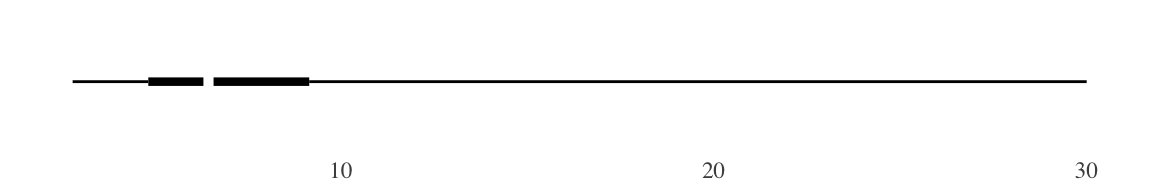
\includegraphics{report_files/figure-latex/unnamed-chunk-2-1.pdf}
\caption{Distribution of public libraries across America by state.}
\end{figure}

\begin{longtable}[]{@{}rrrrrr@{}}
\toprule
Min. & 1st Qu. & Median & Mean & 3rd Qu. & Max.\tabularnewline
\midrule
\endhead
2.8 & 4.67 & 6.44 & 8.04 & 8.81 & 30\tabularnewline
\bottomrule
\end{longtable}

\vspace{10pt}

As is apparent in Figure 1, there is a positive-skew distribution in the
data over the range from 2.797 libraries per 100,000 people to 30.002
libraries per 100,000 people. The positive-skew can also be seen in the
summary statistics for the boxplot, as the mean is greater than the
median. Given that the interquartile range is relatively small in
comparison to the range of the entire data set, there is rather little
variability in terms of the overall distribution of libraries per
100,000 people. Six outlying states, such as Vermont (30.002 libraries
per 100,000 people) and Maine (20.375 libraries per 100,000 people) are
responsible for pulling the skew in the positive direction. On average,
states have 8.037 libraries per 100,000 people as calculated in relation
to the state's population.

Unlike the distribution of libraries by state, the users of such
libraries is approximately normal.

\vspace{20pt}

\begin{figure}[htbp]
\centering
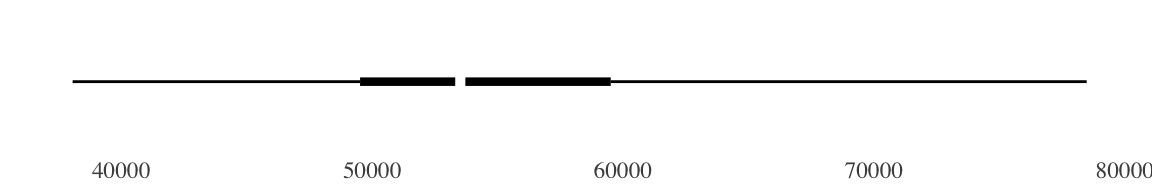
\includegraphics{report_files/figure-latex/unnamed-chunk-4-1.pdf}
\caption{Distribution of library users.}
\end{figure}

\begin{longtable}[]{@{}rrrrrr@{}}
\toprule
Min. & 1st Qu. & Median & Mean & 3rd Qu. & Max.\tabularnewline
\midrule
\endhead
38100 & 49600 & 53500 & 54400 & 59100 & 78500\tabularnewline
\bottomrule
\end{longtable}

\vspace{0pt}

Over the range from 3,8053 to 7,8466 users per 100,000 people, the
distribution is approximately understood due to the difference between
the mean (53,507 users for every 100,000 people) and median (54,413
users for every 100,000 people). Ohio (78,466 users for every 100,000
people) and Minnesota (75,319 users for every 100,000 people) are the
only two outliers in the dataset and lie in the positive direction.

\newpage

\vspace{20pt}

\begin{figure}[htbp]
\centering
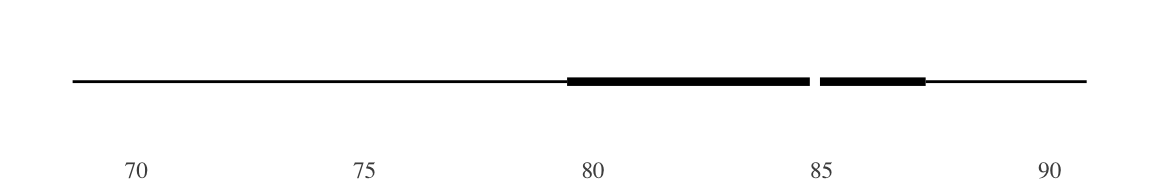
\includegraphics{report_files/figure-latex/unnamed-chunk-6-1.pdf}
\caption{Caption}
\end{figure}

\begin{longtable}[]{@{}rrrrrr@{}}
\toprule
Min. & 1st Qu. & Median & Mean & 3rd Qu. & Max.\tabularnewline
\midrule
\endhead
2.797485 & 4.672557 & 6.435159 & 8.036514 & 8.805816 &
30.00176\tabularnewline
\bottomrule
\end{longtable}

\vspace{10pt}

\vspace{20pt}

\begin{figure}[htbp]
\centering
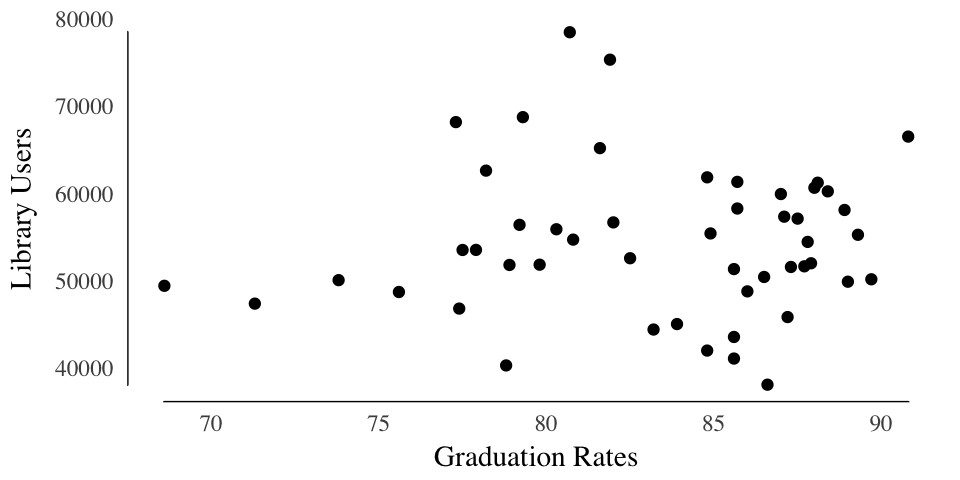
\includegraphics{report_files/figure-latex/unnamed-chunk-8-1.pdf}
\caption{Caption}
\end{figure}

\begin{longtable}[]{@{}rrrrrr@{}}
\toprule
Min. & 1st Qu. & Median & Mean & 3rd Qu. & Max.\tabularnewline
\midrule
\endhead
2.797485 & 4.672557 & 6.435159 & 8.036514 & 8.805816 &
30.00176\tabularnewline
\bottomrule
\end{longtable}

\vspace{10pt}

\newpage




\newpage
\singlespacing 
\end{document}
